% \documentclass[tikz]{standalone}
% \begin{document}
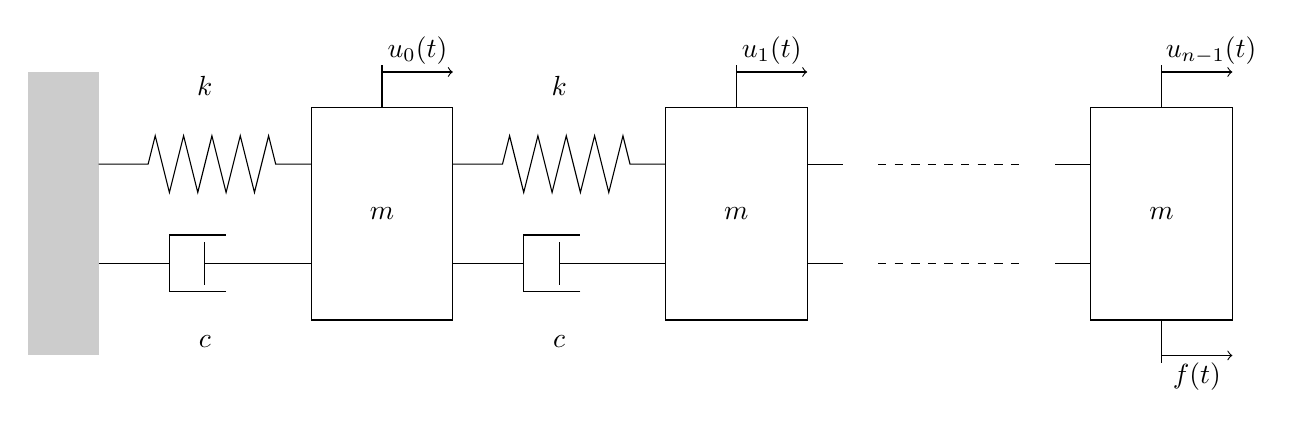
\begin{tikzpicture}[scale=.9]
\fill[black!20] (-1,-2) rectangle (0,2);
\draw (0,.7) -- (.7,.7) -- (.8,1.1) -- (1.0,.3) -- (1.2,1.1) -- (1.4,.3) -- (1.6,1.1) -- (1.8,.3) -- (2.0,1.1) -- (2.2,.3) -- (2.4,1.1) -- (2.5,.7) -- (3.0,.7);
\draw (0,-.7) -- (1,-.7);
\draw (1.8,-1.1) -- (1,-1.1) -- (1,-.3) -- (1.8,-.3); 
\draw (1.5,-1) -- (1.5,-.4);
\draw (1.5,-.7) -- (3,-.7);
\draw (3,-1.5) -- (3,1.5) -- (5,1.5) -- (5,-1.5) -- cycle;
\draw (1.5,-1.8) node  {$c$};
\draw (1.5,1.8) node  {$k$};
\draw (4,0) node {$m$};
\draw (4,1.5) -- (4,2.1);
\draw[->] (4,2) -- (5,2);
\draw (4.5,2.3) node {$u_0(t)$};
\draw (5,.7) -- (5.7,.7) -- (5.8,1.1) -- (6.0,.3) -- (6.2,1.1) -- (6.4,.3) -- (6.6,1.1) -- (6.8,.3) -- (7.0,1.1) -- (7.2,.3) -- (7.4,1.1) -- (7.5,.7) -- (8.0,.7);
\draw (5,-.7) -- (6,-.7);
\draw (6.8,-1.1) -- (6,-1.1) -- (6,-.3) -- (6.8,-.3); 
\draw (6.5,-1) -- (6.5,-.4);
\draw (6.5,-.7) -- (8,-.7);
\draw (8,-1.5) -- (8,1.5) -- (10,1.5) -- (10,-1.5) -- cycle;
\draw (6.5,-1.8) node  {$c$};
\draw (6.5,1.8) node  {$k$};
\draw (9,0) node {$m$};
\draw (9,1.5) -- (9,2.1);
\draw[->] (9,2) -- (10,2);
\draw (9.5,2.3) node {$u_1(t)$};
\draw (10,.7) -- (10.5,.7);
\draw[dashed] (11,.7) -- (13,.7);
\draw (13.5,.7) -- (14,.7);
\draw (10,-.7) -- (10.5,-.7);
\draw[dashed] (11,-.7) -- (13,-.7);
\draw (13.5,-.7) -- (14,-.7);
\draw (14,-1.5) -- (14,1.5) -- (16,1.5) -- (16,-1.5) -- cycle;
\draw (15,0) node {$m$};
\draw (15,1.5) -- (15,2.1);
\draw[->] (15,2) -- (16,2);
\draw (15.7,2.3) node {$u_{n-1}(t)$};
\draw (15,-1.5) -- (15,-2.1);
\draw[->] (15,-2) -- (16,-2);
\draw (15.5,-2.3) node {$f(t)$};
\end{tikzpicture}

% \end{document}